\documentclass[11pt]{article}
\usepackage[a4paper,margin=1in]{geometry}
\usepackage{fourier} % Fourier font
\usepackage{xcolor}
\usepackage{tikz}
\usepackage[most]{tcolorbox}
\usepackage{amsthm, amsmath, amssymb}
\usepackage{enumitem}
\usepackage{hyperref}
\usepackage[nameinlink,noabbrev]{cleveref}
\usepackage{titling} 

% Dark mode colors
\definecolor{bgcolor}{HTML}{FFFFFF}
\definecolor{textcolor}{HTML}{000000}
\definecolor{defcolor}{HTML}{E86873}
\definecolor{thmcolor}{HTML}{0A9396}
\definecolor{lemcolor}{HTML}{94D2BD}
\definecolor{corcolor}{HTML}{9B4AF7}
\definecolor{probcolor}{HTML}{EE9B00}
\definecolor{excolor}{HTML}{21E933}

% Background and text color
\pagecolor{bgcolor}
\color{textcolor}

% No paragraph indentation
\setlength{\parindent}{0pt}
\setlength{\parskip}{0.7em}

% Theorem box styles
\tcbset{
  enhanced,
  colback=bgcolor,
  colframe=thmcolor,
  coltext=white,
  coltitle=white,
  fonttitle=\bfseries,
  boxrule=0.7pt,
  left=1em,
  right=1em,
  top=0.7em,
  bottom=0.7em,
  before skip=10pt,
  after skip=10pt,
}

% Theorem environments with colored boxes
\newtcbtheorem[number within=section]{thm}{Theorem}{
  colframe=thmcolor, colback=thmcolor!15!bgcolor
}{thm} % The 'thm' here is the *prefix* for the label

\newtcbtheorem[number within=section]{defn}{Definition}{
  colframe=defcolor, colback=defcolor!15!bgcolor
}{def} % The 'def' here is the *prefix* for the label

\newtcbtheorem[number within=section]{lem}{Lemma}{
  colframe=lemcolor, colback=lemcolor!15!bgcolor
}{lem}

\newtcbtheorem[number within=section]{cor}{Corollary}{
  colframe=corcolor, colback=corcolor!15!bgcolor
}{cor}

\newtcbtheorem[number within=section]{prob}{Problem}{
  colframe=probcolor, colback=probcolor!15!bgcolor
}{prob}

\newtcbtheorem[number within=section]{ex}{Example}{
  colframe=excolor, colback=excolor!15!bgcolor
}{ex}

% Proof environment 
\renewenvironment{proof}[1][\proofname]{%
  \par\pushQED{\qed}\normalfont\topsep6pt \trivlist
  \item[\hskip\labelsep\itshape #1.]\ignorespaces
}{%
  \popQED\endtrivlist\addvspace{6pt}
}

% Cleveref name formats for tcolorbox environments
\crefname{thm}{theorem}{theorems}
\Crefname{thm}{Theorem}{Theorems}

\crefname{def}{definition}{definitions}
\Crefname{def}{Definition}{Definitions}

\crefname{lem}{lemma}{lemmas}
\Crefname{lem}{Lemma}{Lemmas}

\crefname{cor}{corollary}{corollaries}
\Crefname{cor}{Corollary}{Corollaries}

\crefname{prob}{problem}{problems}
\Crefname{prob}{Problem}{Problems}

\crefname{ex}{example}{examples}
\Crefname{ex}{Example}{Examples}

\usepackage{mathtools}
\usepackage{tikz}
\usetikzlibrary{automata, positioning}

\title{\huge{Mat210 Advanced Discrete Mathematics Notes}}
\author{\LARGE{Thobias Høivik}}
\date{\Large{Fall 2025}}

\begin{document}
\maketitle

\newpage
\tableofcontents

\newpage

\section{Pre-Semester Start – Cardinality}

The following chapter contains notes based on what I think the  
course will cover in the first week (week 33).  
According to the syllabus, cardinality is mentioned early,  
so this section will review some basics.

\begin{defn}{Cardinality}{}
Let \( A \) and \( B \) be sets. We say \( A \) and \( B \) have the same \emph{cardinality}, written \( |A| = |B| \), if there exists a bijection \( f : A \to B \). If no such bijection exists, the sets have different cardinalities.
\end{defn}

\begin{ex}{}{}
Let \(A = \{1,2\}\), \(B = \{3,4\}\). While this is a trivial example, we can show that there are as many elements in \(A\) as in \(B\) by constructing a function \(f:A \to B\) and showing that \(f\) is a bijection.

\begin{proof}[Proof that \(|A| = |B|\)]
Let \(f:A \to B\) be defined by
\[
f(n) = n + 2.
\]
Let \(x, y \in A\) and suppose \(f(x) = f(y)\). Then
\begin{align*}
f(x) &= f(y) \\
x + 2 &= y + 2 \\
x &= y.
\end{align*}
Thus, \(f\) is injective.

Now let \(b \in B\). Then \(b - 2 \in A\), since \(B = \{3,4\}\) and subtracting 2 yields values in \(A = \{1,2\}\). So for every \(b \in B\), there exists \(a = b - 2 \in A\) such that \(f(a) = b\). Hence, \(f\) is surjective.

Since \(f\) is both injective and surjective, it is a bijection, and therefore \(|A| = |B|\).
\end{proof}
\end{ex}

\begin{defn}{Finite and Infinite Sets}{}
A set \( A \) is \emph{finite} if there exists a natural number \( n \in \mathbb{N} \) such that \( |A| = |\{1, 2, \dots, n\}| \). Otherwise, \( A \) is \emph{infinite}.
\end{defn}

\begin{defn}{Countably Infinite}{}
A set \( A \) is \emph{countably infinite} if there exists a bijection \( f : \mathbb{N} \to A \). A set is \emph{countable} if it is finite or countably infinite.
\end{defn}

\begin{defn}{Uncountable Set}{}
A set \( A \) is \emph{uncountable} if it is not countable; that is, there does not exist a bijection from \( \mathbb{N} \) to \( A \).
\end{defn}

\begin{ex}{}{}
The set \( \mathbb{R} \) is famously uncountable, as is rigorously demonstrated in any introductory analysis course (e.g., via Cantor’s diagonal argument).
\end{ex}

\begin{defn}{Power Set}{}
Let \( A \) be a set. The \emph{power set} of \( A \), denoted \( \mathcal{P}(A) \), is the set of all subsets of \( A \).
\end{defn}

\begin{thm}{Cantor's Theorem}{}
For any set \( A \), we have \( |\mathcal{P}(A)| > |A| \). In particular, there is no surjection from \( A \) onto \( \mathcal{P}(A) \).

\begin{proof}
It suffices to show that there cannot exist a surjective function \( f : A \to \mathcal{P}(A) \).

Suppose, for contradiction, that such a surjective function \( f \) exists. Define the set
\[
B = \{ a \in A \mid a \notin f(a) \}.
\]
Then \( B \subseteq A \), so \( B \in \mathcal{P}(A) \). Since \( f \) is surjective, there exists \( b \in A \) such that \( f(b) = B \).

We now ask: is \( b \in B \)?

\begin{itemize}
\item If \( b \in B \), then by the definition of \( B \), \( b \notin f(b) = B \), a contradiction.
\item If \( b \notin B \), then by the definition of \( B \), \( b \in f(b) = B \), again a contradiction.
\end{itemize}

In either case, we reach a contradiction. Therefore, our assumption that \( f \) is surjective must be false. Hence, there is no surjection from \( A \) onto \( \mathcal{P}(A) \), and so
\[
|\mathcal{P}(A)| > |A|.
\]
\end{proof}
\end{thm}

After showing that the power set is strictly larger, we usually demonstrate that
\[
|\mathcal{P}(A)| = 2^{|A|} > |A|
\]
even for infinite sets. However, for infinite cardinals, exponentiation behaves differently than for finite numbers.  
For example, \( 2^{\aleph_0} = \mathfrak{c} = |\mathbb{R}| \).

\begin{prob}{}{}
Prove that \( |\mathbb{N}| = |\mathbb{Z}| \), assuming \( 0 \in \mathbb{N} \).
\end{prob}

\begin{proof}[Proof of Problem 1.1]
We will construct a bijection \( f : \mathbb{N} \to \mathbb{Z} \).

Define:
\[
f(n) =
\begin{cases}
\frac{n}{2} & \text{if } n \text{ is even} \\
-\frac{n + 1}{2} & \text{if } n \text{ is odd}
\end{cases}
\]

We first show that \( f \) is injective. Suppose \( f(x) = f(y) \).

\textbf{Case 1:} Both \( x \) and \( y \) are even.  
Then:
\[
\frac{x}{2} = \frac{y}{2} \Rightarrow x = y.
\]

\textbf{Case 2:} Both \( x \) and \( y \) are odd.  
Then:
\[
-\frac{x + 1}{2} = -\frac{y + 1}{2} \Rightarrow x + 1 = y + 1 \Rightarrow x = y.
\]

\textbf{Case 3:} One is even, one is odd.  
Then \( f(x) \in \mathbb{Z}_{\geq 0} \), \( f(y) \in \mathbb{Z}_{< 0} \), so \( f(x) \neq f(y) \).  
Hence, \( f \) is injective.

Now we show that \( f \) is surjective. Let \( z \in \mathbb{Z} \).  
We find \( n \in \mathbb{N} \) such that \( f(n) = z \):

\textbf{Case 1:} \( z \geq 0 \).  
Then let \( n = 2z \). Since \( z \in \mathbb{Z}_{\geq 0} \), \( n \in \mathbb{N} \), and \( f(n) = z \).

\textbf{Case 2:} \( z < 0 \).  
Then let \( n = -2z - 1 \).  
Since \( z \in \mathbb{Z}_{< 0} \), \( n \in \mathbb{N} \), and:
\[
f(n) = -\frac{n + 1}{2} = -\frac{(-2z - 1 + 1)}{2} = -\frac{-2z}{2} = z.
\]

In both cases, such an \( n \in \mathbb{N} \) exists, so \( f \) is surjective.

Thus, \( f \) is a bijection and \( |\mathbb{N}| = |\mathbb{Z}| \).
\end{proof}

\newpage 
\section{Tasks from 7.4}
\begin{prob}{Task 17}{}
    Show that $\mathbb Q$ is dense along the number line 
    by showing that given two rational numbers 
    $r_1$ and $r_2$ with $r_1 < r_2$, there exists 
    a rational number $x$ such that $r_1 < x < r_2$. 
\end{prob}

\begin{proof}
    Let $r_1, r_2 \in \mathbb Q$ such that $r_1 < r_2$. 
    Consider that average of these numbers 
    \begin{align*}
        x &= \frac{r_1 + r_2}{2} \\ 
          &= \frac{\frac{a}{b} + \frac{c}{d}}{2} \\ 
          &= \frac{a + c}{2bd}
    \end{align*}
    Clearly, $x$ is a rational number since if $a,b,c,d \in \mathbb Z$
    then $a + c \in \mathbb Z$ and $2bd \in \mathbb Z$. 
    Furthermore 
    \begin{align*}
        2r_1 < r_1 + r_2 &\Rightarrow r_1 < \frac{r_1 + r_2}{2} = x \\ 
        r_1 + r_2 < 2r_2 &\Rightarrow \frac{r_1 + r_2}{2} = x < r_2
    \end{align*}
    Thus we have that $x$ is a rational number satisfying 
    the desired property. 
    Hence $\mathbb Q$ is dense along the number line.
\end{proof}

\begin{prob}{Task 26}{}
    Prove that any uncountably infinite set $A$ has a countably 
    infinite
    subset.
\end{prob}

\begin{proof}
    Let $A$ be a set such that $|A| > \aleph_0$.
    To construct a countably infinite subset we proceed by induction
    as follows: 

    Let $a_0 \in A$ be the first element.
    Then for our next element choose some element 
    $a_1 \in A \setminus \{a_0\}$. We know $A \setminus \{a_0\}$ is 
    non-empty since $A$ is infinite.
    If we have $n$ elements in our subset take the subsequent 
    element to be
    $$ 
        a_{n+1} \in A \setminus \{a_0, a_1, \dots, a_n\}
    $$ 
    As mentioned earlier, $A$ take away $\{a_1, \dots, a_n\}$ 
    leaves a non-empty set and $a_{n+1}$ is an available element 
    of this set, meaning we can introduce it to our subset. 
    Then, by mathematical induction, we get a sequence which 
    is itself a type of subset 
    $\{a_i : i \in \mathbb N\}$. 
    Clearly we can construct a bijection 
    $$ 
        f: \mathbb N \to \{a_i : i \in \mathbb N\}
    $$
    such that $f(i) = a_i$. 
    Note that this procedure of making infinitely many choices, 
    means using a weak form of the Axiom of Choice.
\end{proof}

\begin{prob}{Task 27}{}
    Let $A$ and $B$ be sets such that $|A| = \aleph_0$.  
    Prove that if there exists some $g:A \to B$ surjection, 
    then $B$ is countable.
\end{prob}
\begin{proof}
    We will proceed by proving that if there exists some surjection 
    from one set $\Gamma$ to another set $\Delta$, then 
    $|\Gamma| \geq |\Delta|$. With this it follows that $B$ is 
    countable, assuming the conditions set in the problem description.
    Suppose $\phi: \Gamma \to \Delta$ is surjective, 
    i.e. 
    $$ 
        \forall \delta \in \Delta, \exists \gamma \in \Gamma 
        \text{ s.t } \phi(\gamma) = \delta
    $$ 
    Since we assume $\phi$ is well-defined, 
    $\phi(\gamma)$ goes to one and only one $\delta \in \Delta$. 
    Since $\phi$ is surjective, for any $\delta \in \Delta$ there 
    must be at least one $\gamma$ mapped to $\delta$. As stated, 
    no $\gamma$ can map to more than one $\delta$. 
    Therefore, for each $\delta$ to have some $\gamma$ which 
    maps to it there must be at least as many $\gamma \in \Gamma$
    as there are $\delta \in \Delta$. In other words, 
    $$ 
        |\Gamma| \geq |\Delta| 
    $$
    With this fact, and given that we have sets $A, B$ where 
    $|A| = \aleph_0$ and a surjection $g: A \to B$
    it must be the case that  
    $$ 
        |B| \leq |A| = \aleph_0
    $$ 
    which is what it means to be countable.
    
\end{proof}


\begin{prob}{Task 32}{}
    Prove that the cartesian product of $\mathbb Z$ with itself, 
    $\mathbb Z \times \mathbb Z$, is countably infinite.
\end{prob}
\begin{proof}
    To show that $\mathbb Z^2$ is countably infinite we must show that 
    it is infinite 
    ($|\mathbb Z^2| \geq \aleph_0$), and it is countable 
    ($|\mathbb Z^2| \leq \aleph_0$), in other words, 
    $$|\mathbb Z^2| = \aleph_0$$

    First we show $\mathbb Z^2$ is infinite. This should be obvious 
    since $\mathbb Z$ is infinite, but to demonstrate this 
    rigorously consider the function 
    $\pi_1: \mathbb Z^2 \to \mathbb Z$, 
    defined as follows: 
    $$ 
        \pi_1(a, b) = a 
    $$
    Clearly, $\pi_1$ is well-defined, since $(a,b)$ is mapped to 
    a unique $a \in \mathbb Z$.
    Also, $\pi_1$ is surjective, since for any $a \in \mathbb Z$, 
    there exists an infinite amount of elements in $\mathbb Z^2$ 
    such that $\pi_1(a,b) = a$.
    Thus we have shown that we can project $\mathbb Z^2$ onto 
    an infinite set $\mathbb Z$. Hence $\mathbb Z^2$ is infinite. 
    In other words: $|\mathbb Z^2| \geq \aleph_0 $. 
    
    Now we show that there is a surjection from the naturals to 
    $\mathbb Z^2$.
    First define a bijection \(h:\mathbb{Z}\to\mathbb{N}\) by
    \[
        h(n)=\begin{cases}
            2n, & n\ge0,\\[4pt]
            -2n-1, & n<0.
        \end{cases}
    \]
    Let \(\pi:\mathbb{N}\times\mathbb{N}\to\mathbb{N}\) be the 
    Cantor pairing function
    \[
        \pi(a,b)=\frac{(a+b)(a+b+1)}{2}+b,
    \]
    which is a bijection. Its inverse 
    \(\pi^{-1}:\mathbb{N}\to\mathbb{N}\times\mathbb{N}\) 
    can be written explicitly: for \(n\in\mathbb{N}\) set
    \[
        w=\left\lfloor\frac{\sqrt{8n+1}-1}{2}\right\rfloor,\qquad
        t=\frac{w(w+1)}{2},\qquad
        b=n-t,\qquad a=w-b,
    \]
    so \(\pi^{-1}(n)=(a,b)\).

    Now define \(s:\mathbb{N}\to\mathbb{Z}^2\) by
    \[
        s(n)=\big(h^{-1}(a),\,h^{-1}(b)\big)\quad\text{where }\ 
        (a,b)=\pi^{-1}(n).
    \]
    (Here \(h^{-1}:\mathbb{N}\to\mathbb{Z}\) 
    exists because \(h\) is a bijection.)

    To see \(s\) is surjective, take any \((x,y)\in\mathbb{Z}^2\). 
    Let \(a=h(x)\) and \(b=h(y)\). Put \(m=\pi(a,b)\in\mathbb{N}\). 
    Then \(\pi^{-1}(m)=(a,b)\), hence
    \[
        s(m)=\big(h^{-1}(a),h^{-1}(b)\big)=(x,y).
    \]
    Thus every element of \(\mathbb{Z}^2\) has a preimage under 
    \(s\), so \(s\) is surjective.

    Consequently \(|\mathbb{Z}^2|\le|\mathbb{N}|=\aleph_0\). 
    (Since \(\mathbb{Z}^2\) projects onto \(\mathbb{Z}\), 
    we also have \(|\mathbb{Z}^2|\ge\aleph_0\), so in fact 
    \(|\mathbb{Z}^2| =\aleph_0\).)

\end{proof}

\begin{prob}{Task 38}{}
    Suppose $A_1, A_2,\dots$ is an infinite sequence of countable  
    sets. Prove that 
    $$ 
        \bigcup_{i=1}^\infty A_i
    $$
    is countable.
\end{prob}

\begin{proof}
    We intend to show that the countably infinite union 
    of countable sets is countable.

    Let $A_1, A_2, \dots$ be a sequence of countable sets. 

    Recall that 
    \[
        \bigcup_{i=1}^\infty A_i = 
        \{x : x \in A_i, i \in \mathbb Z_+\}.
    \] 
    Since $A_i$ is countable and $\mathbb Z_+$ is countable,  
    there exists a surjection 
    $g_i : \mathbb Z_+ \to A_i$.  
    Recall also that $\mathbb Z_+ \times \mathbb Z_+$ is countable.
    Therefore if we can construct a surjective 
    $f: \mathbb Z_+ \times \mathbb Z_+ \to \bigcup_{i = 1}^\infty A_i$, 
    it follows that 
    $\bigcup_{i=1}^\infty A_i$ is countable.

    Define $f(n, m) = g_n(m)$, where $g_n$ denotes the surjection 
    from $\mathbb Z_+$ to $A_n$.
    To check surjectivity, let $x \in \bigcup_{i=1}^\infty A_i$. 
    Then there exists some $k \in \mathbb Z_+$ such that $x \in A_k$. 
    Since $g_k$ is surjective, there exists $m \in \mathbb Z_+$ 
    such that $g_k(m) = x$. Hence $f(k, m) = x$.
    Therefore $f$ is surjective.

    Since $\mathbb Z_+ \times \mathbb Z_+$ is countable and $f$ is surjective, 
    it follows that $\bigcup_{i=1}^\infty A_i$ is countable.
\end{proof}

\newpage 
\section{Multiplication principle}
\begin{defn}{Multiplication Principle}{}
    If a task can be performed in a sequence of $k$ steps, 
    and the first step can be performed in $n_1$ ways, 
    the second in $n_2$ ways, and so on, then the entire task 
    can be performed in 
    \[
        n_1 \times n_2 \times \cdots \times n_k
    \]
    ways.
\end{defn}

\begin{thm}{Multiplication Principle}{}
    Suppose an experiment consists of two successive stages. 
    If the first stage can be performed in $m$ ways and, 
    for each of these, the second stage can be performed in $n$ ways, 
    then the experiment can be performed in
    \[
        m \times n
    \]
    ways. More generally, if there are $k$ stages with $n_i$ 
    possible outcomes for stage $i$, then the total number of 
    possible outcomes is
    \[
        \prod_{i=1}^k n_i.
    \]
\end{thm}

\begin{ex}{Outfits}{}
    Suppose you have $3$ shirts and $2$ pairs of pants.
    Each shirt can be paired with any pair of pants, 
    so the total number of possible outfits is
    \[
        3 \times 2 = 6.
    \]
\end{ex}

\begin{ex}{License Plates}{}
    A license plate consists of $3$ letters followed by $3$ digits. 
    There are $26^3$ choices for the letters and $10^3$ 
    choices for the digits. 
    Hence, the total number of license plates is
    \[
        26^3 \times 10^3.
    \]
\end{ex}

\begin{ex}{Coin and Die}{}
    Suppose you flip a coin and then roll a die. 
    The coin has $2$ possible outcomes and the die has $6$. 
    By the multiplication principle, the total number of outcomes is
    \[
        2 \times 6 = 12.
    \]
\end{ex}

\newpage
\section{Addition principle}
\begin{thm}{Addition Principle, Two Sets}{}
Let $A$ and $B$ be finite and disjoint sets. Then
\[
|A \cup B| = |A| + |B|.
\]
\end{thm}

\begin{proof}
By definition of union,
\[
A \cup B = \{x \mid x \in A \text{ or } x \in B\}.
\]
Since $A$ and $B$ are disjoint, every element of $A$ is distinct from every element of $B$.  
Thus, counting the elements of $A$ and the elements of $B$ counts all the elements of $A \cup B$ without overlap.  
Therefore, the total number of elements in $A \cup B$ is $|A| + |B|$.
\end{proof}

\begin{thm}{Addition Principle, General Form}{}
Let $A_1, A_2, \dots, A_n$ be pairwise disjoint finite sets. Then
\[
\left| \bigcup_{i=1}^{n} A_i \right| = \sum_{i=1}^{n} |A_i|.
\]
\end{thm}

\begin{proof}
We proceed by induction on $n$.  
\textbf{Base case:} $n=2$ holds by the previous theorem.  
\textbf{Inductive step:} Assume the statement holds for $n=k$. Consider $n=k+1$. Then
\[
\left| \bigcup_{i=1}^{k+1} A_i \right|
= \left| \left(\bigcup_{i=1}^{k} A_i\right) \cup A_{k+1} \right|.
\]
Since the sets are pairwise disjoint, $\bigcup_{i=1}^{k} A_i$ is disjoint from $A_{k+1}$. Thus, by the two-set addition principle,
\[
\left| \bigcup_{i=1}^{k+1} A_i \right|
= \left| \bigcup_{i=1}^{k} A_i \right| + |A_{k+1}|.
\]
By the induction hypothesis,
\[
\left| \bigcup_{i=1}^{k} A_i \right| = \sum_{i=1}^{k} |A_i|,
\]
so
\[
\left| \bigcup_{i=1}^{k+1} A_i \right| = \sum_{i=1}^{k} |A_i| + |A_{k+1}|
= \sum_{i=1}^{k+1} |A_i|.
\]
Hence, by induction, the theorem holds for all $n \geq 2$.
\end{proof}

\begin{ex}{}{}
A cafeteria offers:
\begin{itemize}
    \item 3 types of sandwiches: ham, turkey, or veggie,
    \item 2 types of salads: Greek or Caesar.
\end{itemize}
A student may choose either a sandwich or a salad, but not both.  

Let $S$ be the set of sandwiches and $T$ the set of salads. Then $|S|=3$, $|T|=2$, and $S \cap T = \varnothing$.  
By the addition principle,
\[
|S \cup T| = |S| + |T| = 3 + 2 = 5.
\]
Thus, the student has $5$ possible choices.
\end{ex}

\begin{ex}{}{}
A college course allows students to choose exactly one project topic from three disjoint categories:
\[
\text{Artificial Intelligence (5 topics)},\quad
\text{Networking (4 topics)},\quad
\text{Databases (6 topics)}.
\]
By the general addition principle, the number of possible project choices is
\[
5 + 4 + 6 = 15.
\]
\end{ex}

\subsection{Addition principle for non-disjoint sets}
Suppose we have sets $A,B$ such that 
$A \cap B \neq \emptyset$. 
Then $|A \cup B| \neq |A| + |B|$ since we would 
count at least one element twice.  
We would have to take away one times the number of 
instances of elements that are in both $A$ and $B$. 

\begin{thm}{}{}
    Suppose $A$ and $B$ are sets such that 
    $A \cap B \neq \emptyset$. 
    Then 
    $$
        |A \cup B| = |A| + |B| - |A \cap B|
    $$
\end{thm}
\begin{proof}
    Let $A,B$ be sets such that $A \cap B = C \neq \emptyset$.
    Then $|A| + |B|$ would be the number of 
    elements in $|A \cup B| + \text{ an extra counting of the 
    elements that are common between them, namely } C$.
    Hence we have to take away the number of elements in 
    $C$. 

    I.e. 
    $$ 
        |A \cup B| = |A| + |B| - C = 
        |A| + |B| - |A \cap B|
    $$ 
\end{proof}

\begin{thm}{}{}
    Let $A = A_1 \cup \dots \cup A_n$.
    
    Then 
    $$ 
        |A| = \left|\bigcup_{i=1}^n A_i \right|
        = \displaystyle\sum_{i=1}^{n}|A_i|
        - \displaystyle\sum_{1\leq i < j \leq n}|A_i \cap A_j|
        + \displaystyle\sum_{1\leq i<j<k \leq n}|A_i \cap A_j \cap A_j|
        - \dots + (-1)^{n+1}
    \left|\bigcap_{i=1}^n A_i\right|
    $$ 
\end{thm}

\section{Pigeonhole principle}
\begin{thm}{Pigeonhole principle}{}
    Let $n$ and $m$ be positive integers. If $n > m$, then any function 
    \[
        f : \{1,2,\dots,n\} \to \{1,2,\dots,m\}
    \]
    is not injective. Equivalently, if $n$ objects (pigeons) are placed into $m$ boxes (pigeonholes) with $n > m$, then at least one box contains at least two objects.
\end{thm}

\begin{ex}{}{}
    Suppose there are $13$ people at a party. Each person was born in one of the $12$ months of the year. By the pigeonhole principle, at least two people must share a birth month.
\end{ex}

\begin{ex}{}{}
    Consider $27$ pairs of socks distributed among $26$ drawers. By the pigeonhole principle, at least one drawer must contain at least two pairs of socks.
\end{ex}

\begin{ex}{}{}
    Let $S$ be a set of $6$ integers. If we reduce each integer modulo $5$, we obtain elements in $\{0,1,2,3,4\}$. Since there are $6$ integers and only $5$ possible remainders, by the pigeonhole principle, at least two integers in $S$ must have the same remainder when divided by $5$.
\end{ex}

\newpage 
\section{Permutations}
Roughly speaking, a permutation is a re-arangement of 
the order of a set of ordered items. If we consider the set 
$S = \{1,2,3\}$, then we impose some sort of ordering: 
$$ 
    ABC
$$ 

Then we consider 
$$ 
    BAC
$$  
as a permutation of those letters.

\begin{thm}{}{}
    The number of permutations of a set with $n \in \mathbb Z_+$ 
    elements, 
    is  
    $$ 
        n! = \displaystyle\prod_{i=1}^n i 
    $$ 
\end{thm}

\begin{thm}{}{}
    The number of $r$ permutations of a set with $n$ elements is 
    $$ 
        P(n,r) = \frac{n!}{(n-r)!}
    $$ 
\end{thm}

\newpage
\section{Combinations}
\begin{defn}{Combination}{}
    Let $0 \leq r \leq n$. An r-combination of a set 
    with $n$ elements is a subset with $r$ elements.
\end{defn}

\begin{ex}{}{}
    Let $A = \{a,b,c,d,e\}$. 

    $0$-comb: $\emptyset$

    $1$-comb: $\{a\},\{b\},\dots,\{e\}$

    $2$-comb: $\{a,b\}, \{a,c\}, \dots, \{d,e\}$

    and so on.
\end{ex}

\subsection{Ordered and unordered selection}
In an ordered selection, order matters.

In an unordered selection, order does not matter.

For instance, if we consider an example where we have 
a collection of $5$ numbere objects to collect where $2$ 
are red and $3$ are blue, and we collect them without 
adding them back to the pile, how many ways can you 
collect all $5$ objects. 

This scenario is akin to laying out the objects one after 
the other, meaning it is the same as permuting 
$5$ objects. Hence 
\[
    5! = 120 
\]

If we decide that we do want to put back the objects after 
collecting them we get 
$$ 
    5^5 = 3250
$$ 

If we decided that only the red objects the answer would become 
the number of $2$-permutations of a set containing $5$ elements. 
I.e. 
$$ 
    P(5,2) = \frac{5!}{(5-2)!} = 20
$$ 

\begin{thm}{}{}
    The number of subsets of size $r$ ($r$-combination) of a 
    set with $n$ elements is given by 
    $$ 
        \binom{n}{r} = nCr = \frac{n!}{r!(n-r)!}
    $$ 
\end{thm}

\begin{thm}{Permutations of sets with like elements}{}
    Let a set of $n$ elements consisting of 
    \begin{enumerate}
        \item $n_1$ elements of type $1$
        \item $n_2$ elements of type $2$

            \quad\vdots

        \item $n_k$ elements of type $k$
    \end{enumerate} 

    Then the number of combinations is given by 
    $$ 
    \binom{n}{n_1}\binom{n-n_1}{n_2} \dots \binom{n-n_1-\dots-n_{k-1}}{n_k} 
    = \displaystyle\prod_{i = 1}^k 
    \binom{n - \displaystyle\sum_{j=1}^{i-1}n_j}{n_i}
    = \frac{n!}{n_1!n_2!\cdots n_k!}
    $$ 
\end{thm}

\newpage 
\section{R-combinations with repetition}
Suppose we have a container with $4$ marbles, red, green, blue 
and black. We draw $3$ of them, putting back 
each marble such that each time we draw, the container 
has all $4$ marbles. 

\begin{defn}{}{}
    A $r$-combination with repetition of a set $X$ with $n$ 
    elements is an unordered selection of $r$ elements 
    from $X$ with repetition. 
\end{defn}

It turns out, a problem like this is analogous to 
making a string in the following manner. 
\begin{align*}
    \begin{array}{c|c|c|c}
        Black & Red & Green & Blue
        \\ 
        \hline 
        xx & & & x 
    \end{array}
\end{align*}

In string format: xx|||x. 
This corresponds to choosing $2$ black and $1$ blue. 
Now the problem reduces to: "how many ways can we 
choose 3 elements out of a set of 6 elements?". 
In other words 
$$ 
    \binom{6}{3}
$$  

\begin{thm}{}{}
    The number of $r$-combinations from a set with 
    $n$ elements with repetition is 
    $$ 
        \binom{n-1+r}{r}
    $$ 
\end{thm}

\newpage 
\section{Pascal's formula and the binomial theorem}


\textbf{Formula.}

$$ 
    \binom{n}{r} = \binom{n}{n-r}
$$ 

\begin{proof}
    \begin{align*}
        \binom{n}{r} = \frac{n!}{r!(n-r)!} 
                     = \frac{n!}{(n-r)!(n-(n-r))!} 
                     = \binom{n}{n-r}
    \end{align*}
\end{proof}

\textbf{Pascal's formula.}

\[
    \binom{n+1}{r} = \binom{n}{r-1} + \binom{n}{r}
\]


\begin{thm}{Binomial theorem}{}
    In any field $\mathbb F$ of characteristic $0$, 
    we have for $a,b\in \mathbb F, n \in \mathbb N$:
    $$ 
        (a+b)^n = \displaystyle\sum_{k = 0}^{n} \binom{n}{k}a^{n-k}b^k
    $$ 
\end{thm}

\newpage 
\section{Finite automata}

\begin{defn}{Finite Automaton}{}
A \textbf{deterministic finite automaton (DFA)} is a 5-tuple
\[
A = (Q, \Sigma, \delta, q_0, F)
\]
where:
\begin{itemize}
  \item $Q$ is a finite set of states,
  \item $\Sigma$ is a finite input alphabet,
  \item $\delta : Q \times \Sigma \to Q$ is the transition function,
  \item $q_0 \in Q$ is the start state,
  \item $F \subseteq Q$ is the set of accepting (final) states.
\end{itemize}
\end{defn}

\begin{defn}{Language of a DFA}{}
The \textbf{language recognized} by a DFA $A$ is
\[
L(A) = \{\, w \in \Sigma^* \mid \delta^*(q_0, w) \in F \,\},
\]
where $\delta^*$ is the natural extension of $\delta$ to strings.
\end{defn}

\begin{ex}{A simple automaton}{}
Consider the DFA $A$ over $\Sigma = \{0,1\}$ that accepts all strings ending in $1$.

\[
Q = \{q_0, q_1\}, \quad F = \{q_1\}
\]

\begin{center}
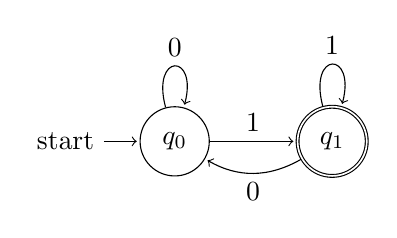
\begin{tikzpicture}[shorten >=1pt, node distance=2cm, on grid, auto]
  \node[state, initial] (q0) {$q_0$};
  \node[state, accepting, right of=q0] (q1) {$q_1$};
  \path[->]
    (q0) edge [loop above] node {0} ()
         edge node {1} (q1)
    (q1) edge [loop above] node {1} ()
         edge [bend left] node {0} (q0);
\end{tikzpicture}
\end{center}
\end{ex}

\subsection{Equivalence of Automata}

\begin{defn}{Nondeterministic Finite Automaton (NFA)}{}
An \textbf{NFA} is a 5-tuple $(Q, \Sigma, \delta, q_0, F)$ where
\[
\delta : Q \times \Sigma \to 2^Q.
\]
The transition function may map to \emph{sets} of states, allowing multiple possible transitions.
\end{defn}

\begin{thm}{Equivalence of DFA and NFA}{}
For every NFA $N$, there exists a DFA $D$ such that
\[
L(D) = L(N).
\]
\end{thm}

\begin{proof}
The proof follows the \textit{subset construction} (or \textit{powerset construction}).  
Each state in the DFA corresponds to a subset of states of the NFA.  
Transitions are defined according to the union of possible NFA transitions under the same input symbol.
\end{proof}

\begin{cor}{Closure under Determinization}{}
The class of regular languages is closed under the determinization process.  
Thus, every language recognized by an NFA is also recognized by a DFA.
\end{cor}

\subsection{Regular Languages}

\begin{defn}{Regular Language}{}
A language $L \subseteq \Sigma^*$ is \textbf{regular} if and only if there exists a DFA (or equivalently, an NFA or regular expression) that recognizes it.
\end{defn}

\begin{thm}{Closure Properties of Regular Languages}{}
Regular languages are closed under the following operations:
\[
\text{union},\; \text{intersection},\; \text{complementation},\; \text{concatenation},\; \text{and Kleene star}.
\]
\end{thm}

\begin{lem}{Closure under Union}{}
If $L_1$ and $L_2$ are regular languages, then $L_1 \cup L_2$ is regular.
\end{lem}

\begin{proof}
Let $A_1$ and $A_2$ be DFAs for $L_1$ and $L_2$.  
Construct a new DFA on the product state space $Q_1 \times Q_2$ with accepting states
\[
F = \{(p, q) \mid p \in F_1 \text{ or } q \in F_2\}.
\]
This automaton recognizes $L_1 \cup L_2$.
\end{proof}

\subsection{Regular expression} 
Let $\Sigma$ be an alphabet. Then we have the following 
recursive definition for regular expressions over 
\(\Sigma\).
\begin{itemize}
    \item \(\emptyset, \lambda\) and the symbols of $\Sigma$ 
        are regular expressions
    \item If \(r,s\) are regular expressions then there 
        concatenation is a regular expression.
    \item If \(r,s\) are regular expressions then 
        $r\mid s$ is a regular expression.
    \item If \(r\) is a reg. exp. then $r^*$ is a reg. exp.
\end{itemize}

\begin{ex}{}{}
    \(\Sigma = \{a,b,c\}\) 

    Regex: \(a \mid (a\mid c)^* \mid (ab)^*\)

    This becomes all strings that are either/or
    \begin{itemize}
        \item \(a\)
        \item any combination of \(a\)'s and \(c\)'s 
        \item any combination of \(ab\)'s
    \end{itemize}
\end{ex}

\end{document}
